\subsection{Reduced model verification}
\subsubsection{Test framework}
As discussed in previous sections, the model is to be used as a state observer for the physical system. The model was reduced from 9 to 7 states in \cref{sec:kalman}. The reduced order model will be refered to as the control model. \\

The control model must initially be tested to accurately estimate the observable states of the full 9-state model. In the test framework, the two models run in parallel, with the control signals $u$ equally applied to both systems. The control signals are computed by the controller K, based on the states of the control model. This framework is seen in \cref{fig:sim_modelSS_obs}. \\

Additionally, an Luenberger observer gain $L$ has been designed. Any error between the actual output and estimated output will be multiplied by $L$ and added to the $\dot{\hat{x}}$. If $A-LC$ is stable, this topology will ensure $\hat{y}$ converges to $y$. If the states are observable (which the Kalman Decomposition ensures) and there is no present disturbance then $\hat{x}$ will converge to $x$. If a disturbance is present, the proportional observer gain will not be sufficient to estimate the states, and integral action should be included. For the purpose of these tests however, the error introduced by the disturbance is not handled by integral observer action. \\

The observer poles (the eigenvalues of $(A-LC)$) are chosen to be have the same angle as the closed loop poles (eigenvalues of $(A-BK)$) but with a 5 times larger magnitude. This ensures the observer is always faster then the system dynamics. Resultingly all state information is available by looking at the observer states ($\hat{x}$).\\

For this test, the ambient temperature is set to 20$^{\circ}$C, which is its operating point value, such that not disturbance is present. This is clear by recalling that $\tilde{d} = d-d_o$

\begin{figure}[h!]
	\centering
	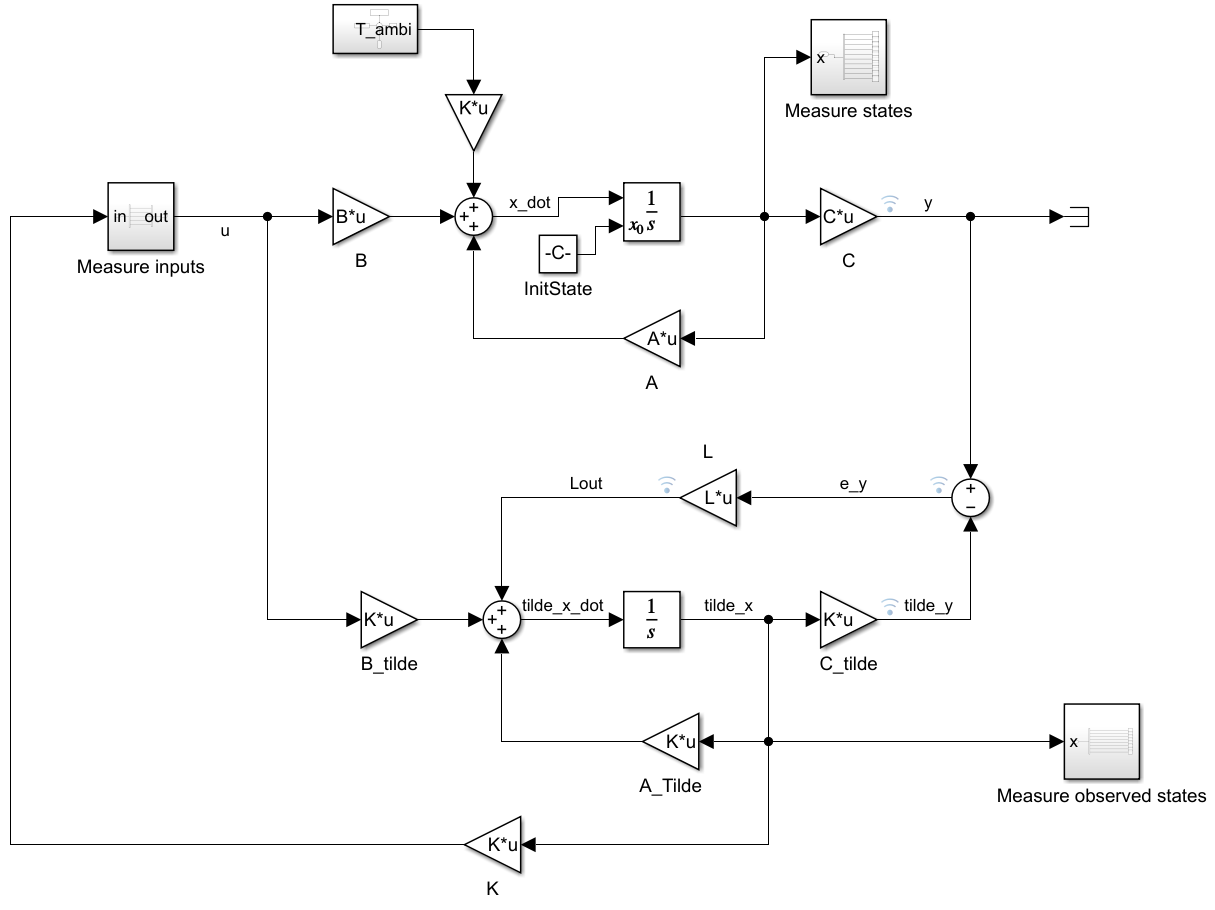
\includegraphics[width=1\textwidth]{Graphics/fig_modelSS_obs.png}
	\caption{The Matlab Simulink simulation model of the linearised system with feedback from Kalman Decomposition observer}
	\label{fig:sim_modelSS_obs}
\end{figure}

\subsubsection{Test results}

For the test all states are initialized with the value 1. This is an arbitrary value, and merely chosen to verify that all states are driven to zero, and the observed state vector $\hat{x}$ converges to $x$. We briefly recall that in this coordinate system $x=0$ physically means $x-x_o = 0 \rightarrow x=x_o$. The control signal u is defined as $u=K\hat{x}$.\\

In \cref{fig:sim_stateInput30h} a plot containing the states and inputs is seen. The simulation has run for 30 hours. In \cref{fig:sim_stateInput1h} the same plot is seen but zoomed in at 1 hour such that the behavior of the states is more easily observed. In \cref{fig:sim_stateObsState1h} The states are compared to the observed states at the same time zoom level as the previous plot. In \cref{fig:sim_stateObsState002h} further zoom is made on the time axis to observe the fast transients in the first seconds of the simulation where the observer converges from the big starting error.


\begin{figure}[h!]
	\centering
	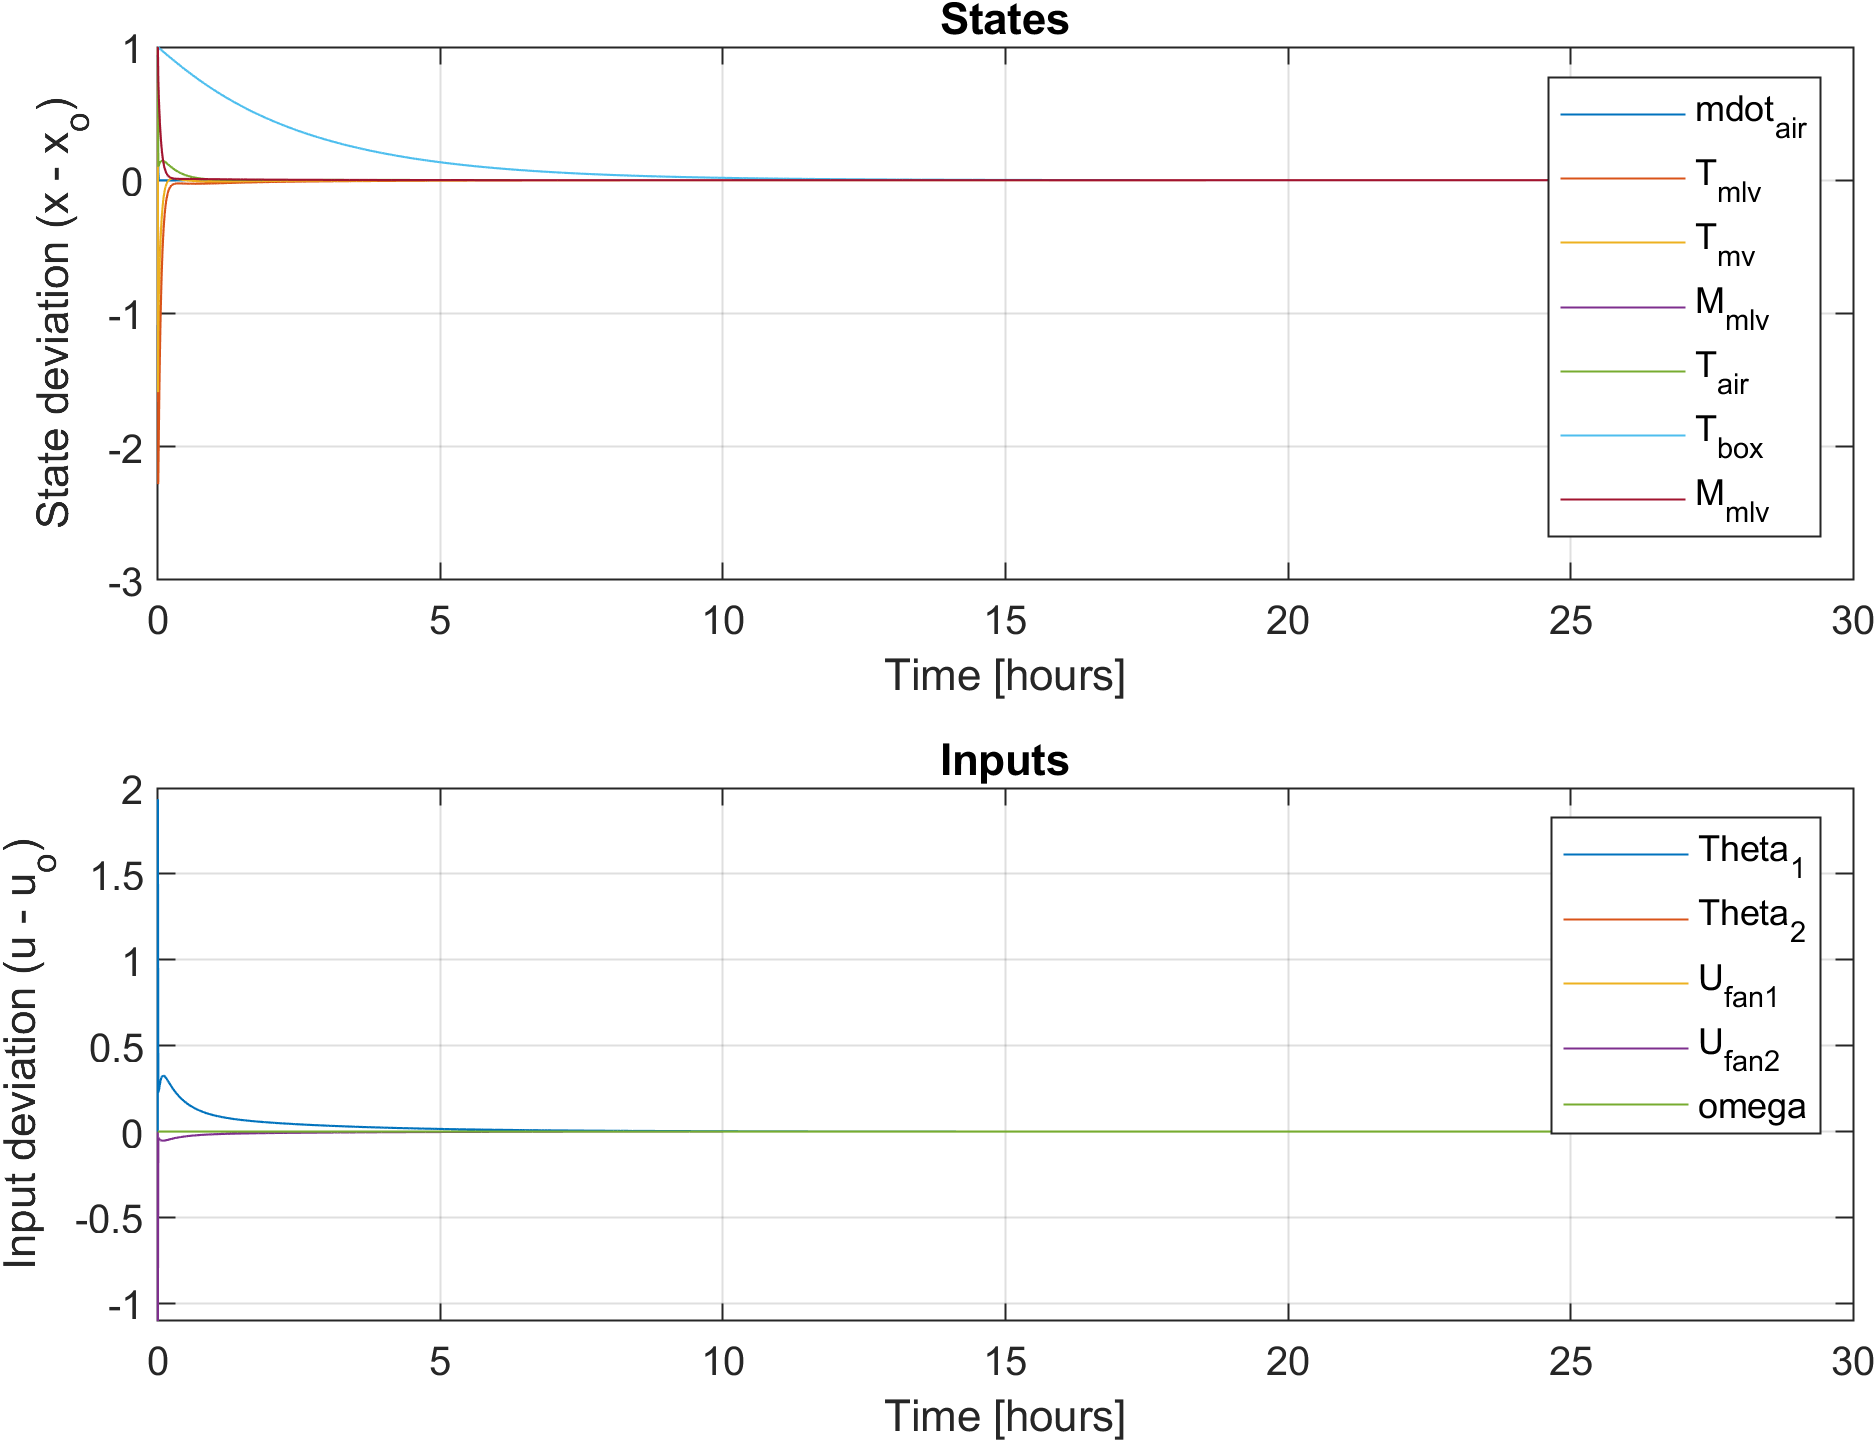
\includegraphics[width=0.7\textwidth]{Graphics/fig_stateInput30h.png}
	\caption{States and inputs plotted for 30 hours. All states settle within an hour except the box temperature which settles in about 7-8 hours}
	\label{fig:sim_stateInput30h}
\end{figure}

\begin{figure}[h!]
	\centering
	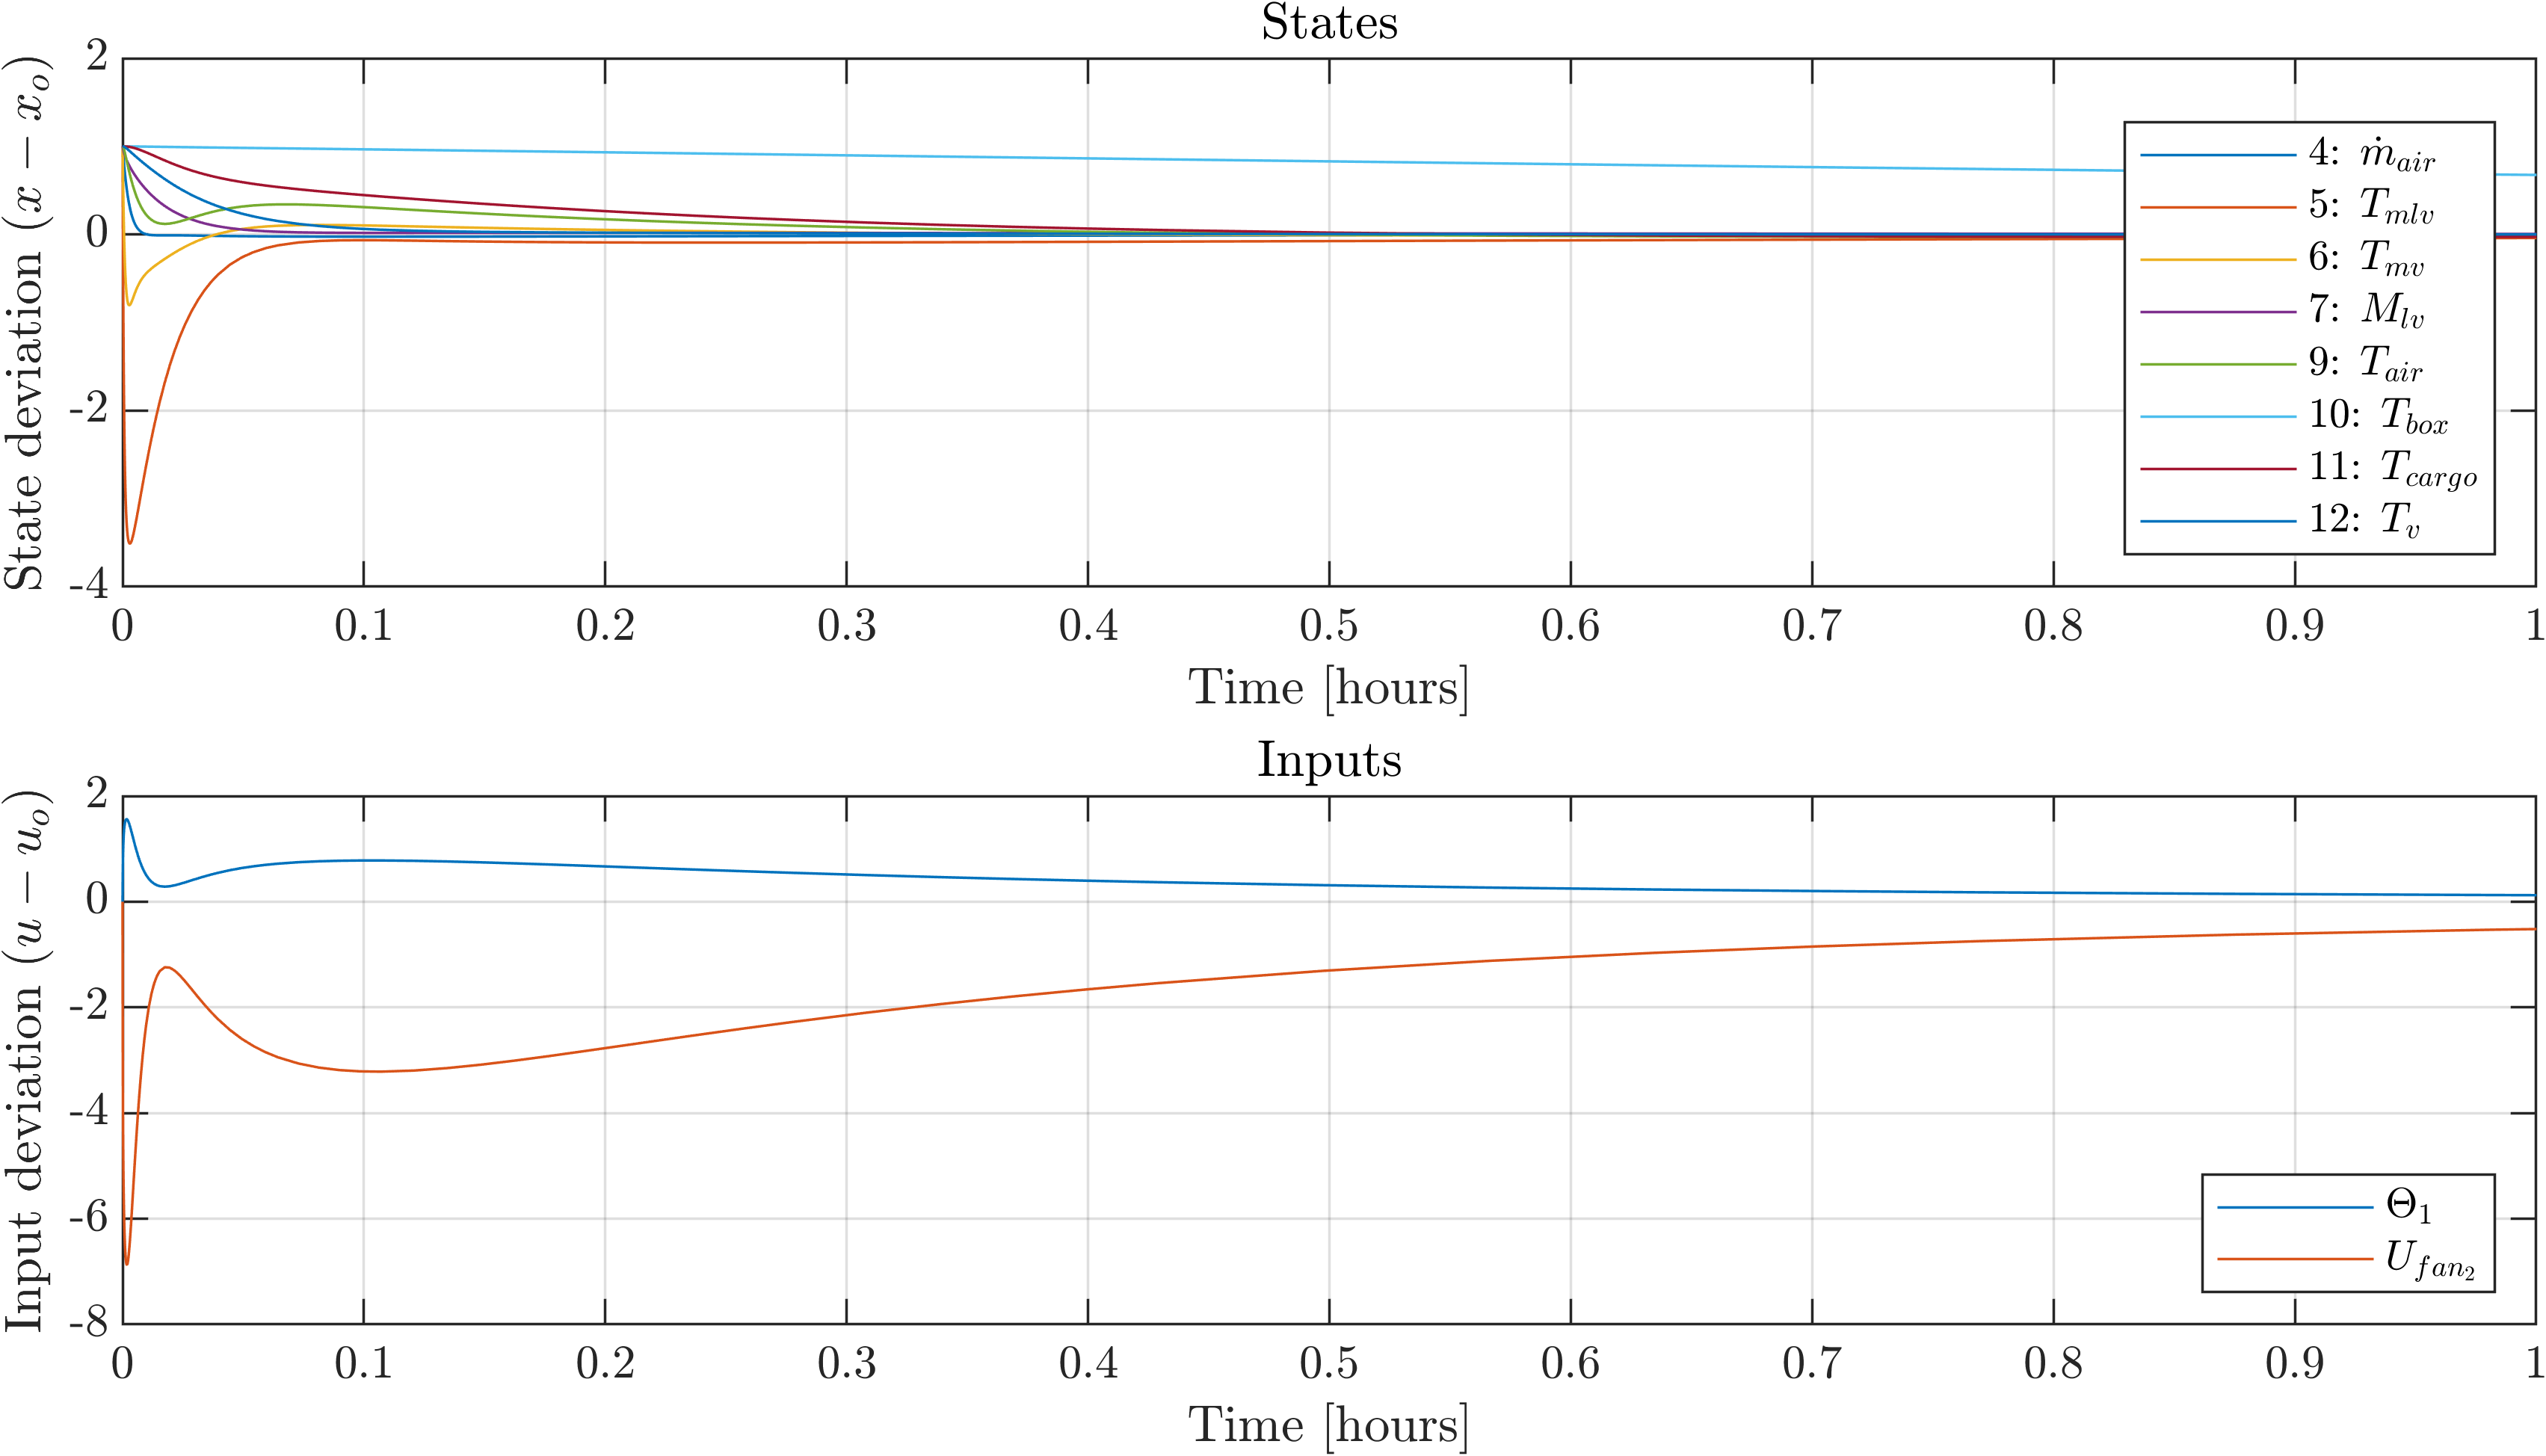
\includegraphics[width=0.7\textwidth]{Graphics/fig_stateInput1h.png}
	\caption{States and inputs plotted for 1 hour.}
	\label{fig:sim_stateInput1h}
\end{figure}

\begin{figure}[h!]
	\centering
	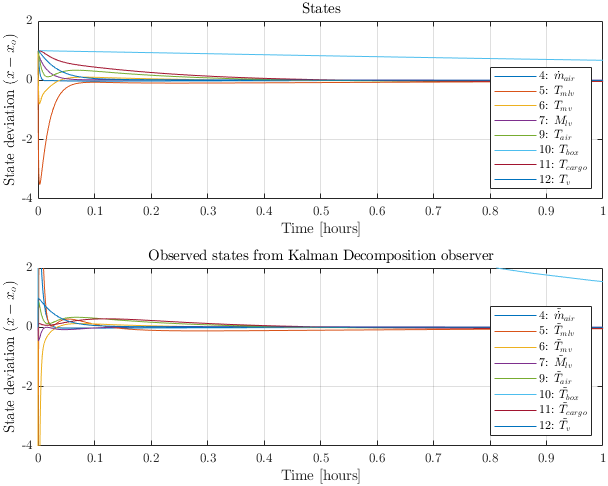
\includegraphics[width=0.7\textwidth]{Graphics/fig_stateObsState1h.png}
	\caption{States and Kalman Decomposition observed states plotted for 1 hour. The estimated box temperature obviously deviates but begins to settle towards the correct state value.}
	\label{fig:sim_stateObsState1h}
\end{figure}

\begin{figure}[h!]
	\centering
	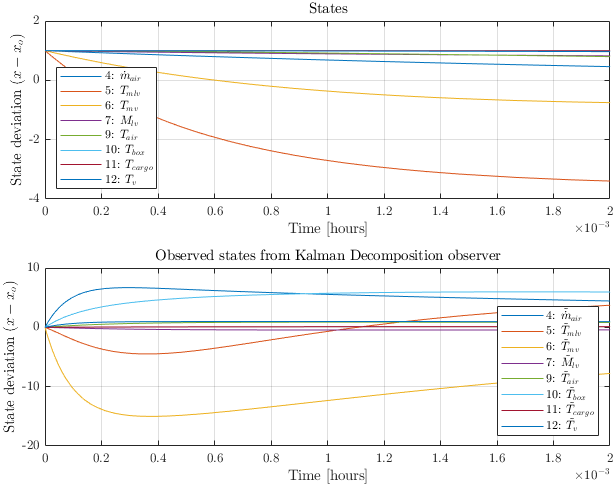
\includegraphics[width=0.7\textwidth]{Graphics/fig_stateObsState002h.png}
	\caption{States and Kalman Decomposition observed states plotted for 0.002 hours. Large deviations observed in the first seconds before observed states converge.}
	\label{fig:sim_stateObsState002h}
\end{figure}
